\documentclass{article}
\usepackage{parskip}
\usepackage{caption}
\usepackage{fancyhdr}
\usepackage{amsmath}
\usepackage{lastpage} 
\usepackage{graphicx} % Required for inserting images
\usepackage[margin=0.9in,top=1in,includefoot]{geometry}
\usepackage{framed} % or, "mdframed"
\usepackage[framed]{ntheorem}
\usepackage{theoremref}
\newframedtheorem{frm-thm}{Theorem}
\makeatletter
\newcommand*{\toccontents}{\@starttoc{toc}}
\makeatother


\newcommand{\RR}{\mathbb{R}}
\newcommand{\NN}{\mathbb{N}}
\newtheorem{thm}{Conjecture}


\begin{document}

\author{Ask Madsen}
\title{Opgaver fra timen d. 23 januar}
\maketitle

\toccontents


\section{Simple ligninger}

I denne opgave skal vi løse simple ligninger. For at løse en simpel ligning flytter vi alle tallene over på den ene side af lighedstegnet og alle x'erne over på den anden side. Til sidst finder vi en værdi for x som er løsningen på vores ligning. Når vå har fundet værdien for x kan vi teste om det er den rigtige værdi ved at indsætte værdien på x's plads i ligningen of tjekke om begge sider af lighedstegnet er ens. Nedenfor er der 3 opgaver med simple ligninger.


\subsection{Opgave}
Løs ligningen $3 + x = 7$.

Vi løser ligningen ved at flytte tallene over på den højre side af lighedstegnet. Vi får

\begin{align*}
3 + x &= 7\\
\Updownarrow \hspace*{14mm} &\\
3 + x - 3 &= 7 - 3 && \text{Trækker 3 fra på begge sider}\\ 
\Updownarrow \hspace*{14mm} &\\
x &= 4
\end{align*}

Når vi løser ligningen får vi at $x = 4$. Vi tjekkerom resultatet er korrekt ved at indsætte $x = 4$ i ligningen

\begin{align*}
3 + x &= 7\\
\Updownarrow \hspace*{8mm} &\\
3 + 4 &= 7 && \text{Indsætter} \hspace*{1mm} x = 4 \hspace*{1mm} \text{på x's plads}\\
\Updownarrow \hspace*{8mm} &\\
7 &= 7
\end{align*}

Da højre og venstre siden af lighedstegnet er ens har vi dermed løst ligningen korrekt. Dette check er ikke nødvendigt, men hvis man er i tvivl om man har løst en ligning korrekt kan man altid tjekke efter ligesom vi har gjort ovenfor.




\subsection{Opgave}
Løs ligningen $4 + 2x = 12$

Vi løser ligningen ved at flytte tallene over på den højre side af lighedstegnet. Vi får

\begin{align*}
4 + 2x &= 12\\
\Updownarrow \hspace*{16mm} &\\
4 + 2x - 4 &= 12 - 4 && \text{Trækker 4 fra på begge sider}\\
\Updownarrow \hspace*{16mm} &\\
2x &= 8\\
\Updownarrow \hspace*{16mm} &\\
\frac{2x}{2} &= \frac{8}{2} && \text{Dividerer med 2 på begge sider så x står alene}\\
\Updownarrow \hspace*{16mm} &\\
x &= 4
\end{align*}

Når vi løser ligningen får vi at $x = 4$. Vi tjekker om resultatet er korrekt ved at indsætte $x = 4$ i ligningen

\begin{align*}
4 + 2x &= 12\\
\Updownarrow \hspace*{12mm} &\\
4 + 2\cdot 4 &= 12 && \text{Indsætter} \hspace*{1mm} x = 4 \hspace*{1mm} \text{på x's plads}\\
\Updownarrow \hspace*{12mm} &\\
4 + 8 &= 12\\
\Updownarrow \hspace*{12mm} &\\
12 &= 12
\end{align*}

Da højre og venstre siden af lighedstegnet er ens har vi dermed løst ligningen korrekt. Dette check er ikke nødvendigt, men hvis man er i tvivl om man har løst en ligning korrekt kan man altid tjekke efter ligesom vi har gjort ovenfor.

\subsection{Opgave}
Løs ligningen $3x - 2 = 7$

Vi løser ligningen ved at flytte tallene over på den højre side af lighedstegnet. Vi får

\begin{align*}
3x - 2 &= 7\\
\Updownarrow \hspace*{16mm} &\\
3x - 2 + 2 &= 7 + 2 && \text{Lægger 2 til på begge sider}\\
\Updownarrow \hspace*{16mm} &\\
3x &= 9\\
\Updownarrow \hspace*{16mm} &\\
\frac{3x}{3} &= \frac{9}{3} && \text{Dividierer med 3 på begge sider så x står alene}\\
\Updownarrow \hspace*{16mm} &\\
x &= 3
\end{align*}

Når vi løser ligningen får vi at $x = 3$. Vi tjekker om resultatet er korrekt ved at indsætte $x = 3$ i ligningen

\begin{align*}
3x - 2 &= 7\\
\Updownarrow \hspace*{12mm} &\\
3\cdot 3 - 2 &= 7 && \text{Indsætter} \hspace*{1mm} x = 3 \hspace*{1mm} \text{på x's plads}\\
\Updownarrow \hspace*{12mm} &\\
9 - 2 &= 7\\
\Updownarrow \hspace*{12mm} &\\
7 &= 7
\end{align*}

Da højre og venstre siden af lighedstegnet er ens har vi dermed løst ligningen korrekt. Dette check er ikke nødvendigt, men hvis man er i tvivl om man har løst en ligning korrekt kan man altid tjekke efter ligesom vi har gjort ovenfor.

\section{Andengradsligninger}

I denne opgave skal vi løse andengradsligninger. For at løse en andengradsligning skal vi bruge følgende theorem

\begin{frm-thm}{Løsning af andengradsligning}\thlabel{anden}

Hvis vi har en andengradsligning på følgende form \hspace*{2cm} $ax^2 + bx + c$

Hvor diskriminanten D beregnes ved \hspace*{4.2cm} $D = b^2 -4ac$

Har andengradsligningen følgende løsninger

\vspace*{4mm}

Hvis $D < 0$ findes der ingen løsninger

Hvis $D = 0$ findes der en løsning \hspace*{4.7cm} $x = \cfrac{-b}{2a}$

Hvis $D > 0$ findes der 2 løsninger \hspace*{4.6cm} $x_1 = \cfrac{-b + \sqrt{D}}{2a}, \hspace*{4mm} x_2 = \cfrac{-b - \sqrt{D}}{2a}$

\end{frm-thm}

\subsection{Opgave}
Løs andengradsligningen $2x^2 + 4x + 2 = 0$

Vi starter med at aflæse a,b og c fra andengradsligningen. Vi ved at a står foran $x^2$, b står foran $x$ og c står for sig selv. Derfor er 
\begin{align*}
a &= 2\\
b &= 4\\
c &= 2
\end{align*}

Når vi har aflæst a, b og c ud fra andengradsligningen beregner vi diskriminanten D. Diskriminanten fortæller os om andengradsligningen har 0, 1 eller 2 løsninger. Vi beregner nu diskriminanten D

\begin{align*}
D = b^2 - 4ac = 4^2 - 4 \cdot 2 \cdot 2 = 16 - 16 = 0
\end{align*}

Da diskriminanten er 0 fortæller Theorem \ref{anden} os at andengradsligningen har 1 løsning. Vi beregner nu løsningen til andengradsligningen

\begin{align*}
x = \frac{-b}{2a} = \frac{-4}{2\cdot 2} = \frac{-4}{4} = -1
\end{align*}

Løsningen til andengradsligningen er dermed $x = -1$. Ligesom i afsnittet om simple ligninger kan vi tjekke om vi har fået det korrekte resultat ved at indsætte $x=-1$ på x's plads i andengradsligningen og se om begge sider af lighedstegnet er ens.

\begin{align*}
2x^2 +4x + 2 &= 0\\
\Updownarrow \hspace*{36mm} &\\
2\cdot (-1)^2 + 4\cdot (-1) + 2 &= 0 && \text{Indsætter} \hspace{1mm} x=-1 \hspace*{1mm} \text{på x's plads}\\
\Updownarrow \hspace*{36mm} &\\
2\cdot 1 -4 + 2 &= 0\\
\Updownarrow \hspace*{36mm} &\\
-2 + 2 &= 0\\
\Updownarrow \hspace*{36mm} &\\
0 &= 0
\end{align*}

Da begge sider af lighedstegnet er ens har vi altså fundet den korrekte løsning til andengradsligningen. Det er ikke nødvendigt at tjekke om man har fået den rigtige løsning men hvis man er i tvivl kan man lave det samme tjek som vi har gjort ovenfor.

Når vi i denne opgave løser andengradsligning  $2x^2 +4x + 2 = 0$ finder vi de x værdier hvor vores parabel $f(x) = 2x^2 +4x + 2$ rammer/skærer x-aksen. I vores tilfælde rammer/skærer vores parabel x aksen når $x = -1$. Nedenfor kan i se dette ilustreret grafisk ved at indtegne parablen $f(x) = 2x^2 + 4x + 2$ i geogebra. Det eneste sted parablen rører x-aksen er præcis når $x=-1$.

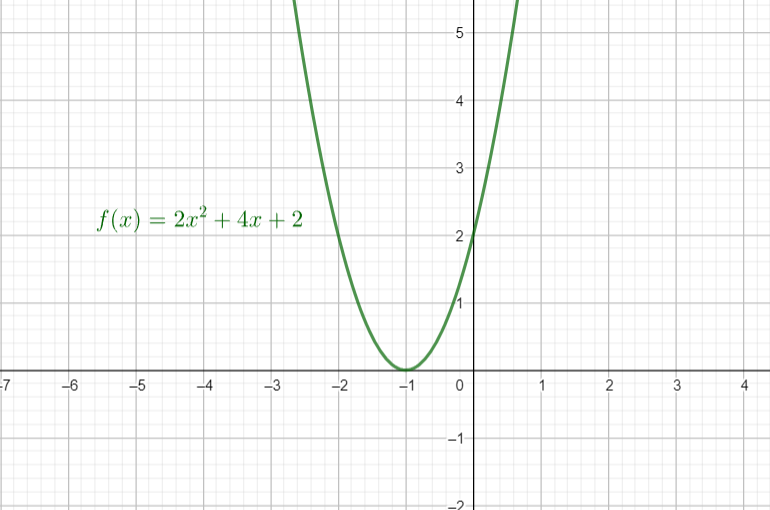
\includegraphics[scale=0.7]{img_1}

\section{Brøkregning}

\subsection{Brøkregneregler}

Det første emne vi kommer til at gennemgå er brøkregneregler. Vi skal lære addition af brøker, subtraktion af brøker, hvordan vi ganger og dividerer brøker og til sidst hvordan vi forkorter brøker. 

En brøk består af 2 tal, det øverste tal kaldes for tælleren og det nederste tal for nævneren. Når vi adderer 2 brøker gælder følgende regler

\begin{frm-thm}{Addition og subtraktion af brøker}\thlabel{add_sub}


Hvis 2 brøker har samme nævner b er additionen og subtraktionen af de 2 brøker givet ved
\[ \frac{a}{b} + \frac{c}{b} = \frac{a + c}{b}   \]
\[\frac{a}{b} - \frac{c}{b} = \frac{a - c}{b}\]

Hvis 2 brøker ikke har samme nævner er deres addition givet ved
\[ \frac{a}{b} + \frac{c}{d} = \frac{a\cdot d + c \cdot b}{b \cdot d} \]
\[\frac{a}{b} - \frac{c}{d} = \frac{a\cdot d - c\cdot b}{b \cdot d} \]
\end{frm-thm}

Vi vil nu gennemgå en række eksempler på hvordan vi laver addition og subtraktion af 2 brøker.

\subsubsection*{Eksempel 1: Addition med ens nævnere}

Vi får givet følgende brøker $\frac{2}{3}$ og $\frac{5}{3}$ og bliver bedt om at bestemme $\frac{2}{3} + \frac{5}{3}$. Da de 2 brøker har fælles nævner siger theorem \ref{add_sub} at vi skal gøre følgende
\begin{align*}
\frac{2}{3} + \frac{5}{3} = \frac{2 + 5}{3} = \frac{7}{3}
\end{align*}

Resultatet af additionen er dermed $\frac{7}{3}$.

\subsubsection*{Eksempel 2: Subtraktion med ens nævnere}

Vi får givet følgende brøker $\frac{2}{3}$ og $\frac{1}{3}$ og bliver bedt om at bestemme $\frac{2}{3} - \frac{1}{3}$. Da de 2 brøker har fælles nævnere siger theorem \ref{add_sub} at vi skal gøre følgende

\begin{align*}
\frac{2}{3} - \frac{1}{3} = \frac{2 - 1}{3} = \frac{1}{3}
\end{align*}

Resultatet af subtraktionen er dermed $\frac{1}{3}$

\subsubsection*{Eksempel 3: Addition med forskellige nævnere}

Vi får givet følgende brøker $\frac{2}{3}$ og $\frac{4}{5}$ og bliver bedt om at bestemme $\frac{2}{3} + \frac{4}{5}$. Da de 2 brøker ikke har fælles nævnere siger theorem \ref{add_sub} at vi skal gøre følgende

\begin{align*}
\frac{2}{3} + \frac{4}{5} = \frac{2\cdot 5 + 4\cdot 3}{3\cdot 5} = \frac{10 + 12}{15} = \frac{22}{15}
\end{align*}

Resultatet af additionen er dermed $\frac{22}{15}$

\subsubsection*{Eksempel 4: Subtraktion med forskellige nævnere}

Vi får givet følgende brøker $\frac{2}{3}$ og $\frac{4}{5}$ og bliver bedt om at bestemme $\frac{2}{3} - \frac{4}{5}$. Da de 2 brøker ikke har fælles nævnere siger theorem \ref{add_sub} at vi skal gøre følgende

\begin{align*}
\frac{2}{3} - \frac{4}{5} = \frac{2\cdot 5 - 4\cdot 3}{3\cdot 5} = \frac{10 - 12}{15} = \frac{-2}{15} = -\frac{2}{15}
\end{align*}


Når vi ganger et tal på en brøk, ganger 2 brøker sammen eller dividerer 2 brøker gælder følgende regler

\begin{frm-thm}{Multiplikation og division af brøker}\thlabel{mult_div}
Hvis vi ganger tallet a ind på en brøk ganger vi a ind i tælleren
\[a\cdot \frac{b}{c} = \frac{a\cdot b}{c}\]

Ganger vi 2 brøker med hinanden ganger vi deres tællere og nævnere sammen
\[\frac{a}{b} \cdot \frac{c}{d} = \frac{a\cdot c}{b\cdot d} \]

Dividerer vi 1 brøk med en anden kan vi i stedet gange med den omvendte brøk (dvs vi bytter om på tælleren og nævneren i den ene brøk)

\[\frac{a}{b} : \frac{c}{d} = \frac{a}{b} \cdot \frac{d}{c}\]
\end{frm-thm}

Vi vil nu gennemgå en række eksempler på hvordan vi kan bruge de ovenstående regler

\subsubsection*{Eksempel 5: Multiplikation af konstant og brøk}

Vi får givet konstanten $4$ og brøken $\frac{3}{5}$ og bliver bedt om at bestemme $4\cdot \frac{3}{5}$. Når vi ganger et tal på en brøk siger theorem \ref{mult_div} at vi skal gøre følgende

\begin{align*}
4\cdot \frac{3}{5} = \frac{4\cdot 3}{5} = \frac{12}{5}
\end{align*}

Resultatet af multiplikationen er dermed $\frac{12}{5}$


\subsubsection*{Eksempel 6: Multiplikation af 2 brøker}

Vi får givet de 2 brøker $\frac{2}{3}$ og $\frac{4}{5}$ og bliver bedt om at bestemme $\frac{2}{3} \cdot \frac{4}{5}$. Når vi ganger 2 brøker sammen siger theorem \ref{mult_div} at vi skal gøre følgende

\begin{align*}
\frac{2}{3} \cdot \frac{4}{5} = \frac{2\cdot 4}{3\cdot 5} = \frac{8}{15}
\end{align*}

Resultatet af multiplikationen er dermed $\frac{8}{15}$

\subsubsection*{Eksempel 7: Divison af 2 brøker}

Vi får givet de 2 brøker $\frac{2}{3}$ og $\frac{4}{5}$ og bliver bedt om at bestemme $\frac{2}{3} : \frac{4}{5}$. Når vi dividerer en brøk med en anden siger theorem \ref{mult_div} at vi skal gøre følgende

\begin{align*}
\frac{2}{3} : \frac{4}{5} = \frac{2}{3} \cdot \frac{5}{4} = \frac{2\cdot 5}{3\cdot 4} = \frac{10}{12}
\end{align*}

Resultatet af divisionen er dermed $\frac{10}{12}$

Vi kigger nu på følgende opgaver

\subsection{Opgave: Addition af brøker med fælles nævner}
Beregn $\frac{1}{2} + \frac{3}{2}$.

Da brøkerne har fælles nævner kan vi ifølge Theorem \ref{add_sub} lægge tællerne sammen og vi får

\begin{align*}
\frac{1}{2} + \frac{3}{2} = \frac{1 + 3}{2} = \frac{4}{2} = 2
\end{align*}

Resultatet af additionen er dermed $2$.

\subsection{Opgave: Addition af brøker med forskellige nævnere}
Beregn $\frac{1}{3} + \frac{1}{6}$.

Da brøkerne ikke har fælles nævner, skal vi først forlænge den ene af brøkerne så de får fælles nævner. Da den først brøk har nævneren 3 og den anden brøk nævneren 6, kan brøkerne få fælles nævneren 6 ved at gange 2 på tælleren og nævneren af den første brøk og derefter lægge brøkerne sammen. Vi får dermed

\begin{align*}
\frac{1}{3} + \frac{1}{6} = \frac{2\cdot 1}{2\cdot 3} + \frac{1}{6} = \frac{2}{6} + \frac{1}{6} = \frac{2 + 1}{6} = \frac{3}{6} = \frac{1}{2}
\end{align*}

Resultatet af additionen er dermed $\frac{1}{2}$.

\subsection{Opgave: Subtraktion af bøker med forskellige nævnere}
Beregn $\frac{1}{2} - \frac{1}{4}$.

Da brøkerne ikke har fælles nævnere skal vi forlænge den ene af brøkerne så de får fælles nævner. Da den første brøk har nævneren 2 og den anden nævneren 4, kan brøkerne få fælles nævneren 4 ved at gange 2 på tælleren og nævneren af den første brøk og derefter trække brøkerne sammen. Vi får dermed

\begin{align*}
\frac{1}{2} - \frac{1}{4} = \frac{2\cdot 1}{2\cdot 2} - \frac{1}{4} = \frac{2}{4} - \frac{1}{4} = \frac{2 - 1}{4} = \frac{1}{4}
\end{align*}

Resultatet af subtraktionen er dermed $\frac{1}{4}$.

\subsection{Opgave: Subtraktion af brøker med forskellige nævnere}
Beregn $\frac{3}{4} - \frac{1}{2}$.

Da brøkerne ikke har fælles nævnere skal vi forlænge den ene af brøkerne så de får fælles nævner. Da den første brøk har nævneren 4 og den anden nævneren 2, kan brøkerne få fælles nævneren 4 ved at gange 2 på tælleren og nævneren af den anden brøk og derefter trække brøkerne sammen. Vi får dermed

\begin{align*}
\frac{3}{4} - \frac{1}{2} = \frac{3}{4} - \frac{2\cdot 1}{2\cdot 2} = \frac{3}{4} - \frac{2}{4} = \frac{3-2}{4} = \frac{1}{4}
\end{align*}

Resultatet af subtraktionen er dermed $\frac{1}{4}$.

\subsection{Opgave: Multiplikation af brøker}
Beregn $\frac{2}{1}\cdot \frac{1}{2}$.

For at gange 2 brøker sammen siger Theorem \ref{mult_div} at vi ganger tællerne sammen og nævnerne sammen. Vi får dermed

\begin{align*}
\frac{2}{1}\cdot \frac{1}{2} = \frac{2\cdot 1}{1\cdot 2} = \frac{2}{2} = 1
\end{align*}

Resultatet af multiplilationen er dermed $1$.

\subsection{Opgave: Multiplikation af brøker}
Beregn $\frac{1}{4}\cdot \frac{1}{3}$.

For at gange 2 brøker sammen siger Theorem \ref{mult_div} at vi ganger tællerne sammen og nævnerne sammen. Vi får dermed

\begin{align*}
\frac{1}{4}\cdot \frac{1}{3} = \frac{1\cdot 1}{4\cdot 3} = \frac{1}{12}
\end{align*}

Resultatet af multiplikationen er dermed $\frac{1}{12}$.

\subsection{Opgave: Division af brøker}
Beregn $\frac{1}{4}:\frac{1}{3}$.

For at dividere 1 brøk med en anden brøk siger Theorem \ref{mult_div} at vi skal gange med den omvendte brøk. Vi får dermed

\begin{align*}
\frac{1}{4}:\frac{1}{3} = \frac{1}{4} \cdot \frac{3}{1} = \frac{1\cdot 3}{4\cdot 1} = \frac{3}{4}
\end{align*}

Resultatet af divisionen er dermed $\frac{3}{4}$.



\section{Procent regning}

\subsection{Opgave: Procentdel af et tal}
Beregn $11\%$ af 750 kr.

For at beregne en procentdel af et tal, tager vi procentdelen og deler med 100, hvorefter vi ganger med tallet vi skal finde procentdelen af. Vi får

\begin{align*}
\frac{11}{100}\cdot 750 = 82.5
\end{align*}

11 procent af 750 kr er dermed 82.5 kr.

\subsection{Opgave: At beregne et procenttal}
Beregn 7 ud af 103.

For at beregne procenttallet, tager vi delen og dividerer med det hele, hvorefter vi ganger med 100. Vi får

\begin{align*}
\frac{7}{103}\cdot 100 = 6.80
\end{align*}

7 er altså 6.80$\%$ af 103.

\subsection{Opgave: At beregne hele mængden}
Beregn $150 \sim 50\%$.

For at beregne hele mængden, tager vi delmængden og dividerer med procenten hvorefter vi ganger med 100. Vi får

\begin{align*}
\frac{150}{50}\cdot 100 = 300
\end{align*}

Hvis 150 er 50$\%$ af en mængde er hele mængden dermed 300.




\section{Gange og parenteser}

Når vi ganger ind i parenteser, skal vi gange ind på alle ledene i parentesen. To led er enten adskilt af et plus eller minus.

Når vi ganger 2 parenteser sammen, skal vi gange alle ledene fra den første parentes sammen med alle ledene fra den anden parentes.

\subsection{Opgave: Gang ind i parentesen}
Reducer $2(3+a)$.

Vi ganger 2 ind på alle ledene i parentesen dvs vi ganger 2 på 3 og 2 på a. Vi får

\begin{align*}
2(3+a) = 2\cdot 3 + 2a = 6 + 2a
\end{align*}

Resultatet af at gange 2 ind i parentesen er dermed $6 + 2a$

\subsection{Opgave: Gang ind i parentesen}
Reducer $4a(2+a)$.

Vi ganger 4a ind på begge led i parentesen dvs ind på 2 og a. Vi får

\begin{align*}
4a(2+a) = 4a\cdot 2 + 4a\cdot a = 8a + 4a^2
\end{align*}

Resultatet af at gange $4a$ ind i parentesen er dermed $6 + 2a$ da $a\cdot a = a^2$.

\subsection{Opgave: Gang 2 parenteser sammen}
Reducer $(2+a)\cdot (b+1)$.

Vi ganger 2 fra den første parentes ind på b og 1 i den anden parentes og a fra den første parentes ind på 1 og b i den anden parentes. Vi får

\begin{align*}
(2+a)\cdot (b+1) = 2b + 2\cdot 1 + ab + a = 2b + 2 + ab + a
\end{align*}

Resultatet af at gange de 2 parenteser sammen er dermed $2b + 2 + ab + a$.

\subsection{Opgave: Gange 2 parenteser sammen}
Reducer $(a+b)\cdot (3+a)$.

Vi ganger a fra den første parentes ind på 3 og a fra den anden parentes og b fra den første parentes ind på 3 og a fra den anden parentes. Vi får

\begin{align*}
(a+b)\cdot (3+a) = a\cdot 3 + a\cdot a + b\cdot 3 + ba = 3a + a^2 +3b + ba
\end{align*}

Resultatet af at gange de 2 parenteser sammen er dermed $3a + a^2 +3b + ba$.
\end{document}